\documentclass[a4paper,12pt]{article}
\usepackage[a4paper, total={180mm, 272mm}]{geometry}

\usepackage{fontspec}
\setmainfont[Path=fonts/, Extension=.ttf]{ipaexm}

\setlength\parindent{3.5em}
\setlength\parskip{0em}
\renewcommand{\baselinestretch}{1.247}

\usepackage{graphicx}
\graphicspath{{images/}}

\begin{document}

\thispagestyle{empty}

\Large
\noindent \\
Spin Blur Ino\medskip
\par
\normalsize
回転方向に平均値ぼかしを行ないます。\\
\par
初めに、指定あれば Alphaチャンネルに対して処理します。\par
次に、Alphaチャンネルがゼロでないピクセルの RGBを処理します。\par
Alphaチャンネルに処理をしないときは、RGB画像の変化を Alpha値\par
でマスクします。よって、滑らかなエッジは滑らかなままです。\\
\\
-{-}- \ 入力 \ -{-}-\\
Source\par
処理をする画像を接続します。\\
Reference\par
Pixel 毎に効果の強弱をつけるための参照画像を接続します。\\
\\
-{-}- \ 設定 \ -{-}-\\
Center\par
回転の中心位置を指定します。\par
原点は処理をする画像の中心です。カメラの注視点ではありません。\par
単位はミリメートルです。\par
初期値は\textquotedbl 0.0 0.0\textquotedbl で原点位置が中心です。\\
\\
Radius\par
中心からぼかさない範囲を指定します。\par
単位はミリメートルです。\par
0以上の値を入力します。\par
初期値は0で全体にぼかします。\\
\\
Blur\par
ぼかしの強さを調整をします。\par
ぼかしの強さは、回転角度で指定します。\par
最小は0でこのときは何もしません。最大は180です。\par
初期値は1です。\\
\\
Type\par
Accelerator\par
\noindent \hskip 7em Blur角度に対して、\par
\noindent \hskip 7em 外周へ行くほど強くかかります。\par
\noindent \hskip 7em Centerから結果画像の上下高の半分の位置において、\par
\noindent \hskip 7em Blur角度でかかり、その内側では弱くかかり、その外側では\par
\noindent \hskip 7em 強くかかります。

\newpage

\thispagestyle{empty}

\ \vspace{-0.2em}
\par
Uniform\par
\noindent \hskip 7em Centerから近くても遠くても Blur角度一定でかかります。\\
\par
初期値は\textquotedbl Accelerator\textquotedbl です。\\
\\
Alpha Rendering\par
ONで Alphaにも処理をします。\par
OFFのときは、Alpha に処理しませんが、\par
RGB値の変化を Alpha 値でマスクします。\par
初期値は ONです。\\
\\
Anti Alias\par
ジャギーをなくすためにアンチエイリアスを加えた処理を行います。\par
結果はなめらかになりますが時間がかかります。\par
初期値は OFFです。\par
<処理時間参考例>\par
Width=2176 Height=1236 Center=0,0 Radius=0 Blur=3 Alpha=ON\par
Shrink=1\par
\noindent \hskip 7em Type=Accelerator\par
\noindent \hskip 10.5em Anti Alias=OFF 約28sec\par
\noindent \hskip 10.5em Anti Alias=ON \, 約360sec\par
\noindent \hskip 7em Type=Uniform\par
\noindent \hskip 10.5em Anti Alias=OFF 約23sec\par
\noindent \hskip 10.5em Anti Alias=ON \, 約280sec\par
Shrink=3\par
\noindent \hskip 7em Type=Accelerator\par
\noindent \hskip 10.5em Anti Alias=OFF 約5sec\par
\noindent \hskip 10.5em Anti Alias=ON \, 約17sec\par
\noindent \hskip 7em Type=Uniform\par
\noindent \hskip 10.5em Anti Alias=OFF 約4sec\par
\noindent \hskip 10.5em Anti Alias=ON \, 約13sec\\
\\
Reference\par
Pixel 毎に効果の強弱をつけるための参照画像の値の取り方を選択します。\par
入力の\textquotedbl Reference\textquotedbl に画像を接続し、\par
Red/Green/Blue/Alpha/Luminance/Nothingから選びます。\par
この効果をつけたくないときは Nothingを選ぶか、接続を切ります。\par
初期値は Red です。

\newpage

\thispagestyle{empty}

\ \vspace{-0.2em}
\par
\noindent Spin Blur \ \ 参考例

\large
\noindent \begin{picture}(0,0)
\put(170.5,-144.5){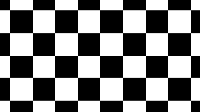
\includegraphics[width=13.3em]{SpinBlurInoOriginalImage}}
\put(92.5,-343){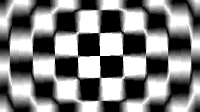
\includegraphics[width=13.3em]{SpinBlurInoUniformBlur11AAOFF}}
\put(314.5,-343){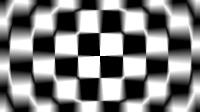
\includegraphics[width=13.3em]{SpinBlurInoUniformBlur11AAON}}
\put(92.5,-486){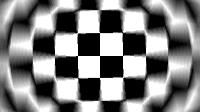
\includegraphics[width=13.3em]{SpinBlurInoAcceleratorBlur11AAOFF}}
\put(314.5,-486){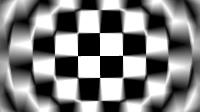
\includegraphics[width=13.3em]{SpinBlurInoAcceleratorBlur11AAON}}
\put(26,-50){\normalsize{元画像}}
\put(26,-67){\normalsize{(200x112pixel)}}
\put(89,-221){\normalsize{Anti Alias \ \ OFF}}
\put(311,-221){\normalsize{Anti Alias \ \ ON}}
\put(26,-249){\normalsize{Uniform}}
\put(26,-267){\normalsize{(Blur\,11.25)}}
\put(26,-382){\normalsize{Accel-}}
\put(26,-400){\normalsize{erator}}
\put(26,-418){\normalsize{(Blur\,11.25)}}
\end{picture}\\[12.65em]

\end{document}